\documentclass[12pt, a4 paper]{report}
\usepackage[T1]{fontenc}
\usepackage[polish]{babel}
\usepackage[utf8]{inputenc}
\usepackage[T1]{fontenc}
\usepackage{titlesec}
\titleformat{\chapter}[display]
  {\normalfont\bfseries}{}{0pt}{\Huge}
\usepackage{ragged2e}
\usepackage{blindtext}
\usepackage{xcolor}
\usepackage{float}
\usepackage{amsmath}
\usepackage{multirow}
\usepackage{graphicx}
\usepackage{caption}
\usepackage{subcaption}
\usepackage{hyperref}
\hypersetup{
    colorlinks=true,
    linkcolor=blue,
    pdftitle={Sprawozdanie V Kacper Piątkowski},
    pdfpagemode=FullScreen,
}
%\usepackage{subfigure}
\usepackage{gensymb}
\usepackage{amssymb}
\usepackage{xcolor}
\usepackage[margin=3.1cm]{geometry}
\titlespacing*{\chapter}{0pt}{-30mm}{40pt}
\usepackage{pgfplots}
\usepgfplotslibrary{units}
\pgfplotsset{width=14cm,compat=1.9}
\usepackage{fancyhdr}
\pagestyle{fancy}
\fancyhf{}
\lhead{Elektronika Cyfrowa}
\rhead{Kacper Piątkowski}
\fancyfoot[C]{\thepage}
\usepackage{colortbl}
\usepackage{karnaugh-map}

\title {Sprawozdanie V\\
{\Large Elektronika Cyfrowa}}
\author{
Kacper Piątkowski\\
Grupa 4\\\\
Prowadzący: dr Szymon Niedźwiecki}
\date{Data laboratoriów: 25.05.2022}
\label{grupa}
\begin{document}

\maketitle

\tableofcontents

\chapter{Wstęp}

\section{Używany sprzęt oraz narzędzia}

\begin{itemize}
    \item Stanowisko - \textbf{7}
    \item Oscyloskop - \textbf{MSO3012}
    \item Generator funkcyjny - \textbf{AFG3022B}
    \item Płytka RLC - \textbf{05}
    \item Multimetr - \textbf{3}
    \item Wartości eksperymentalne oraz wykresy dla charakterystyk częstotliwościowych zostały sporządzone za pomocą programu \textbf{Origin 2022}
\end{itemize}

\section{Jednostki i przedrostki}

\begin{itemize}
    \item 1 Hz (herc) - jednostka miary częstotliwości - 1Hz = $\frac{1}{1s} = 1s^{-1}$
    \item 1 A (amper) - jednostka natężenia prądu elektrycznego - 1A = $\frac{1C}{1s}$
    \item 1 V (wolt) - jednostka potencjału elektrycznego, napięcia elektrycznego i siły elektromotorycznej - 1V = $\frac{1W}{1A}$ ($\frac{wat}{amper}$)
    \item 1 F (farad) - jednostka pojemności elektrycznej - 1F = $\frac{1C}{1V}$ ($\frac{kulomb}{wolt}$)
    \item 1 H (henr) - jednostka indukcyjności - 1H = $\frac{1 Wb}{1 A}$ ($\frac{weber}{amper})$
\end{itemize}

\begin{itemize}
    \item k (kilo) = $10^3$
    \item m (mili) = $10^{-3}$
    \item \micro (micro) = $10^{-6}$
    \item n (nano) = $10^{-9}$
\end{itemize}

\section{Funkcja przejścia T($\omega$)}

Sprzężenie wyjścia z wejściem. T = $\dfrac{odpowiedz}{wymuszenie}.$ \\

\begin{equation}
T(\omega) = \frac{Z_2(\omega)}{Z_1(\omega)+Z_2(\omega)}
\end{equation}
$Z_1/Z_2$ - impedancja

\section{Stała czasowa $\tau$}

\begin{center} $\tau$ = R $\cdot$ C \end{center}
R - rezystancja rezystora \\
C - pojemność kondensatora \\

\section{Czwórnik RC}

Czwórnik RC to:
\begin{itemize}
    \item filtr dolnoprzepustowy
    \item układ całkujący
\end{itemize}

Schemat czwórnika:

\begin{figure}[H]
    \centering
    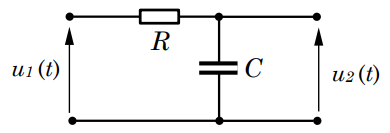
\includegraphics[scale=0.75]{img_wyklad/RC.png}
    \caption{Czwórnik RC}
    \label{fig:RC}
\end{figure}

\section{Czwórnik CR}


Czwórnik CR to: 
\begin{itemize}
    \item filtr górnoprzepustowy
    \item układ różniczkujący
\end{itemize}

Schemat czwórnika:

\begin{figure}[H]
    \centering
    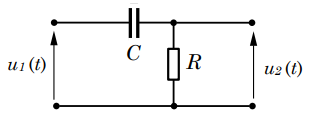
\includegraphics[]{img_wyklad/CR.png}
    \caption{Czwórnik CR}
    \label{fig:CR}
\end{figure}

\section{Czwórnik CLR}

Schemat czwórnika:

\begin{figure}[H]
    \centering
    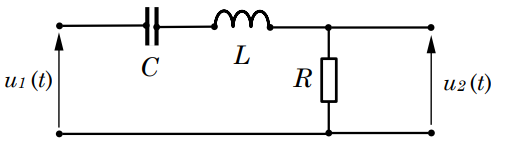
\includegraphics[scale=0.6]{img_wyklad/CLR.png}
    \caption{Czwórnik CLR}
    \label{fig:CLR}
\end{figure}

\section{Charakterystyka amplitudowa}
\label{poprawa:charakterystyka_amplitudowa}

Funkcja określająca zależność $|T|$ od częstości. \\
Charakterystyka amplitudowa dla czwórników CR i RC:
\begin{figure}[H]
    \centering
    \begin{subfigure}[h]{0.45\textwidth}
        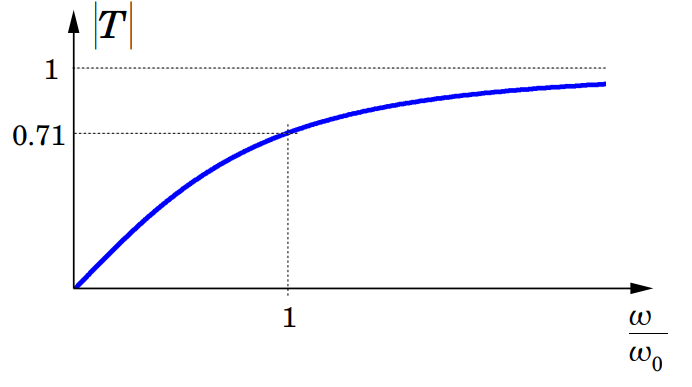
\includegraphics[width=\textwidth]{img_wyklad/teor_amp_CR.png}
        \caption*{Charakterystyka amplitudowa czwórnika CR}
    \end{subfigure}
    \begin{subfigure}[h]{0.45\textwidth}
        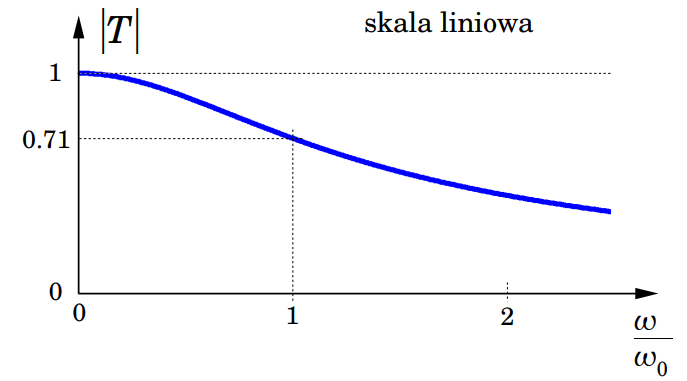
\includegraphics[width=\textwidth]{img_wyklad/teor_amp_RC.png}
        \caption*{Charakterystyka amplitudowa czwórnika RC}
    \end{subfigure}
\end{figure}

\section{Charakterystyka fazowa}
\label{poprawa:charakterystyka_fazowa}

Funkcję określającą zależność $\phi$ od częstości nazywamy charakterystyką fazową. \\
Charakterystyka fazowa dla czwórników CR i RC:
\begin{figure}[H]
    \centering
    \begin{subfigure}[h]{0.45\textwidth}
        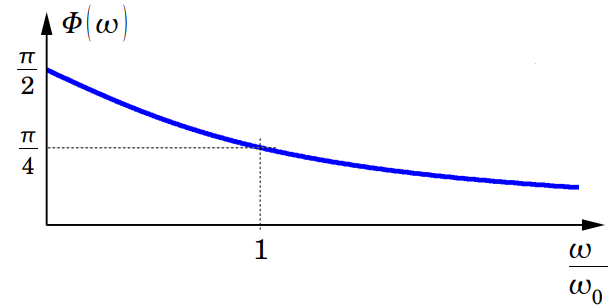
\includegraphics[width=\textwidth]{img_wyklad/teor_faza_CR.png}
        \caption*{Charakterystyka fazowa czwórnika CR}
    \end{subfigure}
    \begin{subfigure}[h]{0.45\textwidth}
        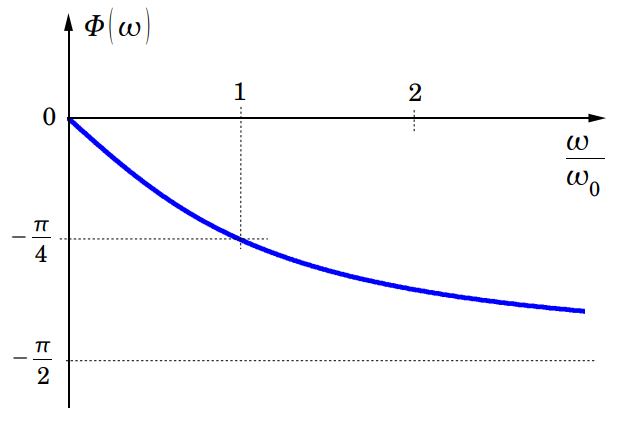
\includegraphics[width=\textwidth]{img_wyklad/teor_faza_RC.png}
        \caption*{Charakterystyka fazowa czwórnika RC}
    \end{subfigure}
\end{figure}

\chapter{Cwiczenie 1}

\section{Obsługa oscyloskopu}
\label{sec:obsluga_oscyloskopu}
\begin{itemize}
\item W celu zapoznania się z możliwościami oscyloskopu włączono kanały \textbf{1} oraz \textbf{2} 
\item Ustawiono skalę pionową za pomocą pokrętła znajdującego się poniżej przycisków do włączenia kanałów odpowiednio na \textbf{500 mV} oraz \textbf{100mV}.
\item Skala pozioma została ustawiona na \textbf{10 ns} a tryb wyzwalania na \textbf{AUTO}.
\item Sygnał \textbf{1} (oznaczony na żółto) przesunięto na $\frac{2}{8}$ wysokości ekranu od góry, zaś \textbf{2} (oznaczony na niebiesko) na środek ekranu.
\item Terminacja została ustawiona na \textbf{50$\Omega$} a sprzężenie na \textbf{DC}

\begin{figure}[h]
    \centering
    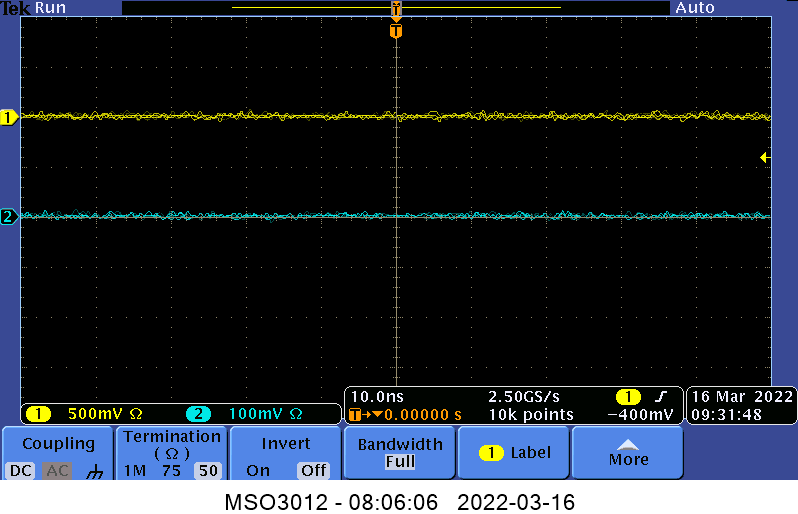
\includegraphics[scale=0.6]{images/1_1_wmenu_smaller.png}
    \caption{Obsługa oscyloskopu - podstawowe ustawienia}
    \label{fig:1_1}
\end{figure}
\end{itemize}

\section{Obsługa generatora funkcyjnego}

W celu zapoznania się z obsługą generatora funkcyjnego podano na oscyloskop sygnał trójkątny o wybranej amplitudzie i częstotliwości.


\begin{itemize}
    \item Za pomocą złącza BNC połączono generator funkcyjny z oscyloskopem na \textbf{kanale 2}.
    \item Włączono \textbf{kanał 2} na oscyloskopie.
    \item Za pomocą generatora funkcyjnego podano \textbf{sygnał trójkątny} wybrany z menu generatora (\textbf{panel Function})
    \item Za pomocą przycisków znajdujących się po prawej stronie wyświetlacza generatora ustawiono \textbf{amplitudę} sygnału na \textbf{1.55V} a jego \textbf{częstotliwość} na \textbf{15kHz}
    \item Powiększono sygnał na oscyloskopie
\end{itemize}

\begin{figure}[h]
    \centering
    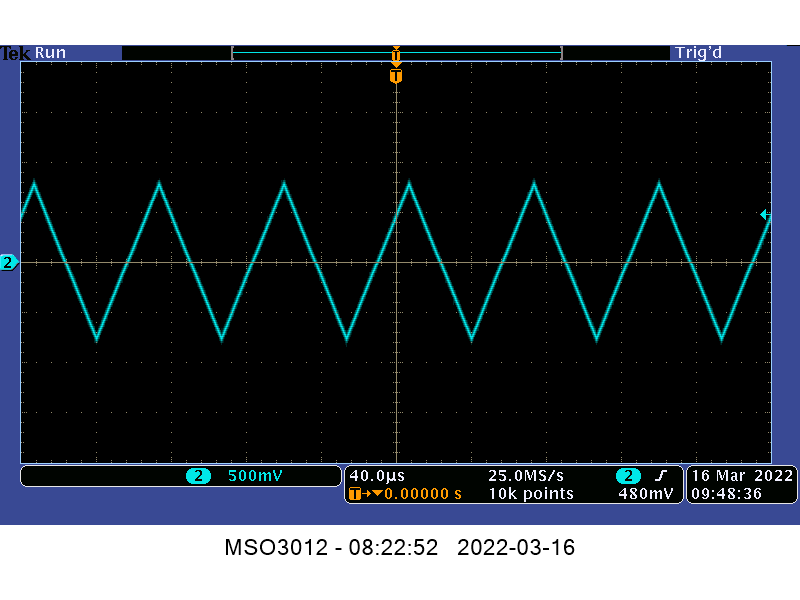
\includegraphics[scale=0.5]{images/1_2.png}
    \caption{Sygnał trójkątny - 1.55V 15kHz}
    \label{fig:trojkat}
\end{figure}

\section{Pomiary}

Dokonano pomiaru podanego przez generator funkcyjny sygnału na \textbf{kanale 2} za pomocą trzech metod.

\label{ad:roznica_2_3-1}
\begin{enumerate}
    \item Metoda określona jako \textbf{pomiar 'na oko'} - za pomocą skali poziomej możemy określić amplitudę podanego sygnału. Skala pozioma została ustawiona na \textbf{500mV} po czym zauważono że sygnał rozpina się na $\frac{3}{8}$ wysokości ekranu. (rys. \ref{fig:trojkat})
    \begin{center}
        Zmierzona wartość = skala $\cdot$ wysokość na ekranie \\
        Zmierzona wartość = 500mV $\cdot$ 3 = 1.5V \\
    \end{center}
        \textcolor{purple}{Różnica wartości wysłanej oraz zmierzonej wyniosła:} 
    \begin{center}
        \textcolor{purple}{$\Delta$ = Teoretyczna wartość - Zmierzona wartość \\ $\Delta$ = |1.55V - 1.5V| =} 0.05V = 50mV
    \end{center}
    
    \item Pomiar za pomocą kursorów - kursory włączono za pomocą przycisku \textbf{Cursors} znajdującego się w lewym górnym rogu menu oscyloskopu. Kursory ustawiono za pomocą pokręteł znajdujących się obok przycisku włączającego kursory (\textbf{multipurpose a/b}) odpowiednio dla mierzonych wartości. W przypadku amplitudy mierzono odległość od najniższego do najwyższego punktu, zaś dla częstotliwości mierzono 1 okres - tutaj od 'dołku' do 'dołku'.
    
    \item Pomiar za pomocą wbudowanych funkcji oscyloskopu - włączone zostały za pomocą przycisku \textbf{Measure} w panelu \textbf{Wave Inspector}, następnie korzystając z nieopisanych przycisków obok wyświetlacza oscylatora wybrano opcję mierzenia \textbf{amplitudy (amplitude)} oraz \textbf{częstotliwości (frequency)} dla \textbf{kanału 2}
\end{enumerate}

\begin{figure}[h]
    \centering
    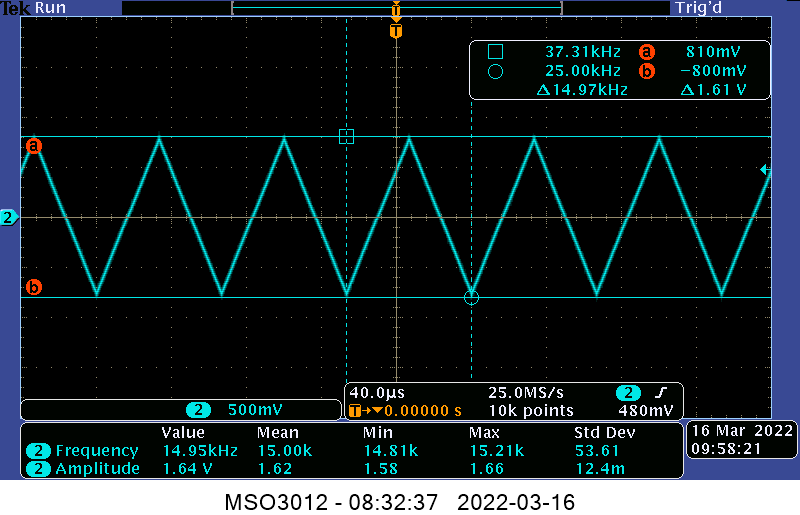
\includegraphics[scale = 0.5]{images/1_3measurement_smaller.png}
    \caption{(\ref{fig:trojkat}) wraz z pomiarami za pomocą kursorów i funkcji wbudowanych}
    \label{fig:trojkat_pomiary}
\end{figure}

\begin{itemize}
    \item W przypadku pomiaru za pomocą kursorów otrzymano następujące wyniki (prawy górny róg \ref{fig:trojkat_pomiary}):
    \begin{center}
        częstotliwość = \textbf{14.97kHz} \\
        amplituda = \textbf{1.61V}
    \end{center}
    \label{ad:roznica_2_3-2}
    \textcolor{purple}{Różnica wartości wysłanych z generatora oraz zmierzonych wyniosła}:
    \begin{center}
        $\Delta$ częstotliwości = \textcolor{purple}{|15kHz - 14.97kHz| =} 0.03kHz = \textbf{30Hz} \\
        $\Delta$ amplitudy = \textcolor{purple}{|1.55V - 1.61V| =} 0.06V = \textbf{60mV}
    \end{center}
    
    \item Pomiar za pomocą funkcji wbudowanych (dolna część \eqref{fig:trojkat_pomiary}):
    \begin{center}
        częstotliwość = \textcolor{purple}{\textbf{15kHz}} \\
        amplituda = \textcolor{purple}{\textbf{1.62V}}
    \end{center}
    \textcolor{purple}{Różnica wartości wysłanych z generatora oraz zmierzonych wyniosła}:
    \label{ad:roznica_2_3-3}
    \begin{center}
        \label{ad:odczyt_2_3}
        $\Delta$ częstotliwości = \textcolor{purple}{|15kHz - 15kHz| = \textbf{0Hz}} \\
        $\Delta$ amplitudy = \textcolor{purple}{|1.55V - 1.62V| = 0.07V} = \textcolor{purple}{\textbf{70mV}}
    \end{center}
\end{itemize}

\section {Zadanie praktyczne - pomiary}

\begin{itemize}
    \item Na \textbf{kanał 1} podano \textbf{sygnał sinusoidalny} o częstotliwości \textbf{15kHz} i amplitudzie \textbf{1V} oraz przesunięciu \textbf{fazowym 30\boldsymbol{\degree}} ($\frac{\pi}{6}$), zaś na\textbf{ kanale 2} podano \textbf{sygnał trójkątny} z poprzedniej części - \textbf{15kHz}, \textbf{1.55V}
    \item Dokonano pomiarów za pomocą kursorów oraz funkcji wbudowanych
\end{itemize}


\begin{itemize}
    \item Za pomocą funkcji wbudowanych w oscyloskopie zmierzono przesunięcie fazowe między \textbf{1} kanałem a \textbf{2}. Zmierzona wartość wyniosła \textbf{31.58}\boldsymbol{\degree}.\\
    \label{ad:roznica_2_4}
    Różnica wartości wyniosła $\approx$ \textcolor{purple}{|30\degree = 31.58\degree| = } \textbf{1.58}\boldsymbol{\degree}.
    
    \begin{figure}[h]
        \centering
        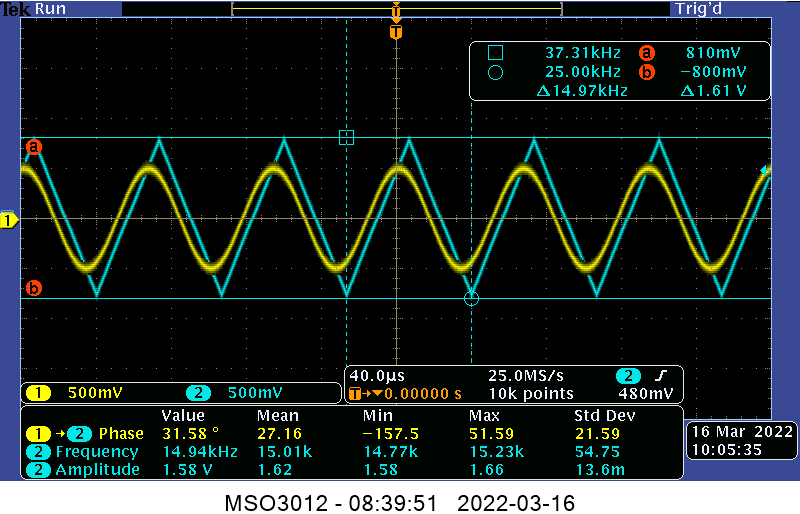
\includegraphics[scale = 0.3]{images/1_4_smaller.png}
        \caption{Sygnał trójkątny oraz sinusoidalny z przesunięciem fazowym 30\degree}
        \label{fig:trójkat_sinus}
    \end{figure}
    
    \item Następnie zmierzono wartości sygnału na \textbf{kanale 1}.
    \begin{center}
        częstotliwość = \textbf{15.06kHz} \\
        amplituda = \textbf{1.1V}
    \end{center}
    \textcolor{purple}{Różnica wartości wysłanych z generatora oraz zmierzonych wyniosła}:
    \begin{center}
        częstotliwość $\approx$ 0.06kHz = \textbf{60Hz} \\
        amplituda $\approx$ 0.1V = \textbf{100mV}
    \end{center}
    
    \begin{figure}[h]
        \centering
        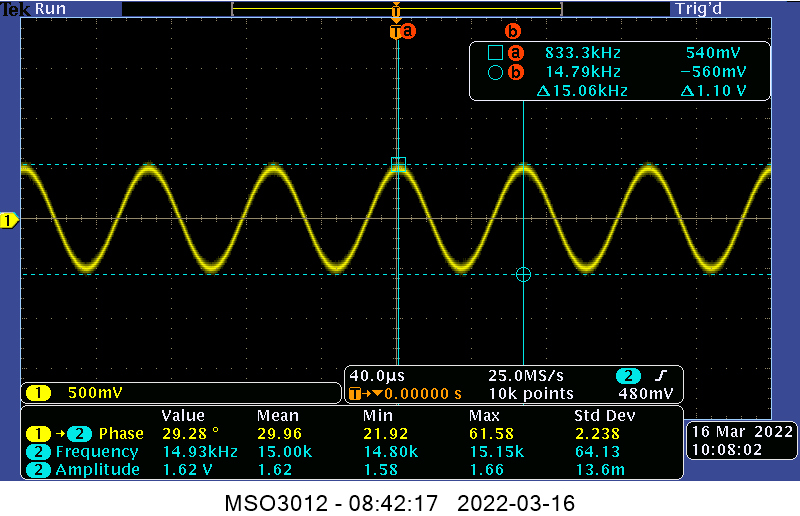
\includegraphics[scale=0.3]{images/1_4sine_smaller.png}
        \caption{Sygnał sinusoidalny wraz z pomiarem za pomocą kursorów}
        \label{fig:pomiar_sinus}
    \end{figure}
\end{itemize}

\section{Podsumowanie}

\begin{itemize}
    \item \textcolor{purple}{Oscyloskop} posiada wiele funkcji ułatwiających dokładny pomiar poprzez dostosowanie skali poziomej oraz pionowej lub zmianę położenia sygnałów
    \label{ad:zla_nazwa_sprzetu_2_5}
    \item Generator funkcyjny w prosty sposób pozwala przesłać na wybrany przez nas kanał sygnał o zadanych parametrach oraz kształcie
    \item Pomiary dokonane za pomocą funkcji wbudowanych jak również kursorów generują w większości niewielkie błędy (różnice między wysłanym sygnałem a zmierzoną wartością)
    \item Posługując się pomiarami za pomocą funkcji wbudowanych w oscyloskopie wykluczamy błędy popełnione przez człowieka, jedynym problemem może być źle skalibrowany sprzęt
    \item Posługując się pomiarami za pomocą kursorów niedokładność pomiarów wynika ze złego ustawienia kursorów, na którą składa się kilka czynników w tym rozdzielczość wyświetlacza na oscylatorze i stopień precyzji kursorów
\end{itemize}

\chapter{Cwiczenie 2}

\section{Krzywe Lissajous}

Korzystając z trybu \textbf{X-Y} oscyloskopu zaobserwowano efekt złożenia dwóch drgań harmonicznych (\textbf{krzywe Lissajous})

\begin{itemize}
    \item Włączono \textbf{tryb X-Y}
    \item Wysłano \textbf{sygnały sinusoidalne} na oba kanały \textcolor{purple}{(o amplitudzie \textbf{1V} oraz bazowej częstotliwości \textbf{15kHz} (w proporcji \textbf{1} oznacza \textbf{15kHz}))}
    \label{ad:dodatkowe_informacje_lissajous}
    \item Ustawiono sygnały w stosunku kolejno: \textbf{1:1, 1:2, 1:3} (częstotliwość) oraz przesunięciu fazowym \textbf{90}\boldsymbol{\degree} ($\frac{\pi}{2}$)
\end{itemize}

\label{ad:teoretyczne_lissajous}
{
    \begin{figure}[H]
        \centering
        \begin{subfigure}[h]{0.45\textwidth}
            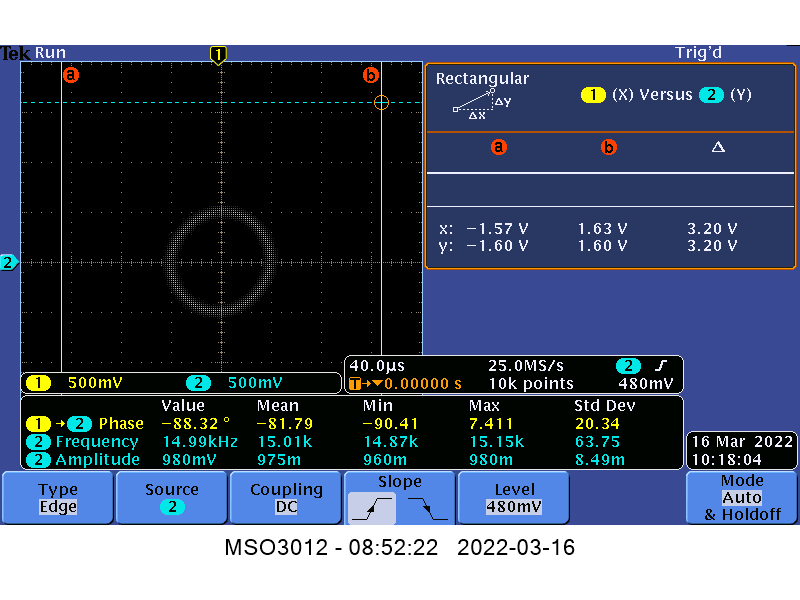
\includegraphics[scale=0.3]{images/1_5_1-1-90.png}
            \caption*{1:1 90$\degree$}
        \end{subfigure}
        \begin{subfigure}[h]{0.45\textwidth}
            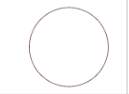
\includegraphics[scale=1.9]{images/theoretical/1-1-90.png}
            \caption*{1:1 90$\degree$ teoretyczna}
        \end{subfigure}
    \end{figure}
    
    \begin{figure}[H]
        \centering
        \begin{subfigure}[h]{0.45\textwidth}
            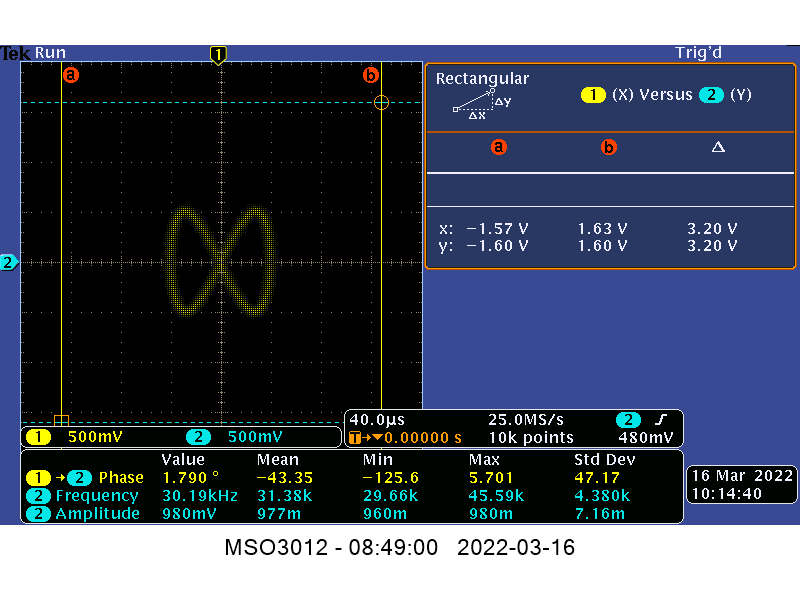
\includegraphics[scale=0.3]{images/1_5_1-2-90.png}
            \caption*{1:2 90$\degree$}
        \end{subfigure}
        \begin{subfigure}[h]{0.45\textwidth}
            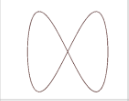
\includegraphics[scale=1.9]{images/theoretical/1-2-90.png}
            \caption*{1:2 90$\degree$ teoretyczna}
        \end{subfigure}
    \end{figure}
    
    \begin{figure}[H]
        \centering
        \begin{subfigure}[h]{0.45\textwidth}
            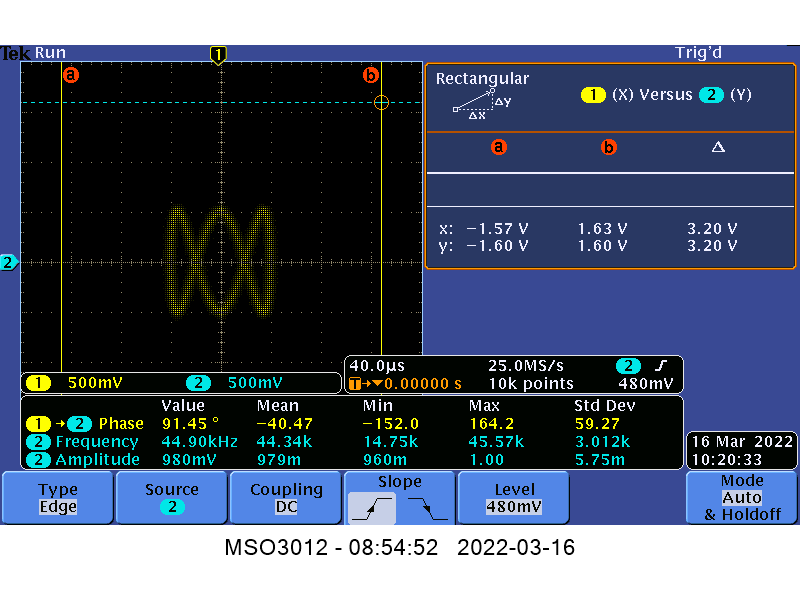
\includegraphics[scale=0.3]{images/1_5_1-3-90.png}
            \caption*{1:3 90$\degree$}
        \end{subfigure}
        \begin{subfigure}[h]{0.45\textwidth}
            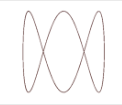
\includegraphics[scale=1.9]{images/theoretical/1-3-90.png}
            \caption*{1:3 90$\degree$ teoretyczna}
        \end{subfigure}
    \end{figure}
}

\begin{itemize}
    \item Następnie ustawiono sygnały w stosunku kolejno: \textbf{1:1, 1:3} (częstotliwość) oraz przesunięciu fazowym \textbf{45}\boldsymbol{\degree} ($\frac{\pi}{4}$)
{
    \begin{figure}[H]
        \centering
        \begin{subfigure}[h]{0.45\textwidth}
            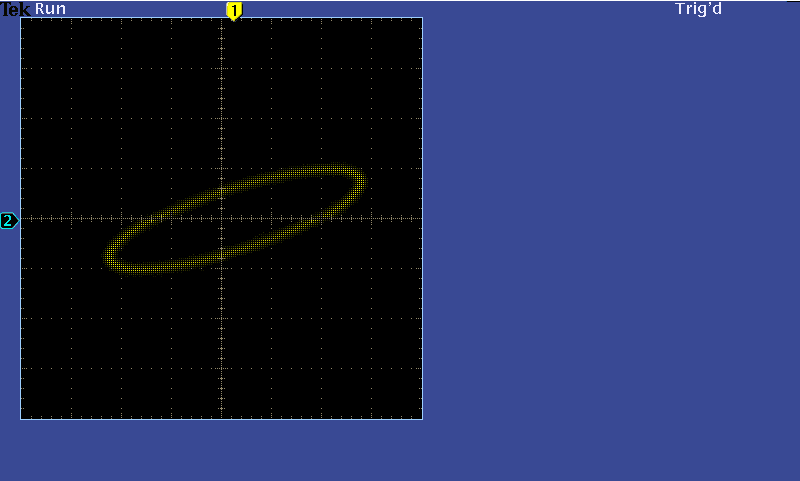
\includegraphics[scale=0.3]{images/zad.5.2.png}
            \caption*{1:1 45$\degree$}
        \end{subfigure}
        \begin{subfigure}[h]{0.45\textwidth}
            
\includegraphics[scale=1.9]{images/theoretical/1-1-45.png}
            \caption*{1:1 45$\degree$ teoretyczna}
        \end{subfigure}
    \end{figure}
    
    \begin{figure}[H]
        \centering
        \begin{subfigure}[h]{0.45\textwidth}
            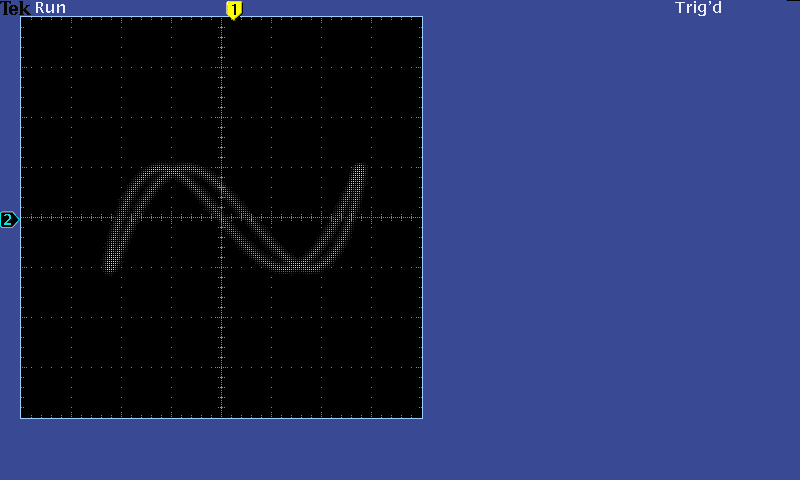
\includegraphics[scale=0.3]{images/zad.5.1.png}
            \caption*{1:3 45$\degree$}
        \end{subfigure}
        \begin{subfigure}[h]{0.45\textwidth}
            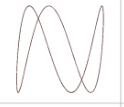
\includegraphics[scale=1.9]{images/theoretical/1-3-45.png}
            \caption*{1:3 45$\degree$ teoretyczna}
        \end{subfigure}
    \end{figure}
}

\end{itemize}

\chapter{Przerzutnik Schmidta}

\section{Budowa układu}

\begin{itemize}
    \item Do budowy układu wykorzystano oporniki \textbf{100}$\boldsymbol{\Omega}$ oraz \textbf{10k}$\boldsymbol{\Omega}$ znajdujących się na płytce, które pozwalają na dynamiczną zmianę oporu.
    \item Za pomocą trójnika doprowadzono sygnał zarówno do płytki, jak i do oscyloskopu.
        \begin{figure}[H]
            \centering
            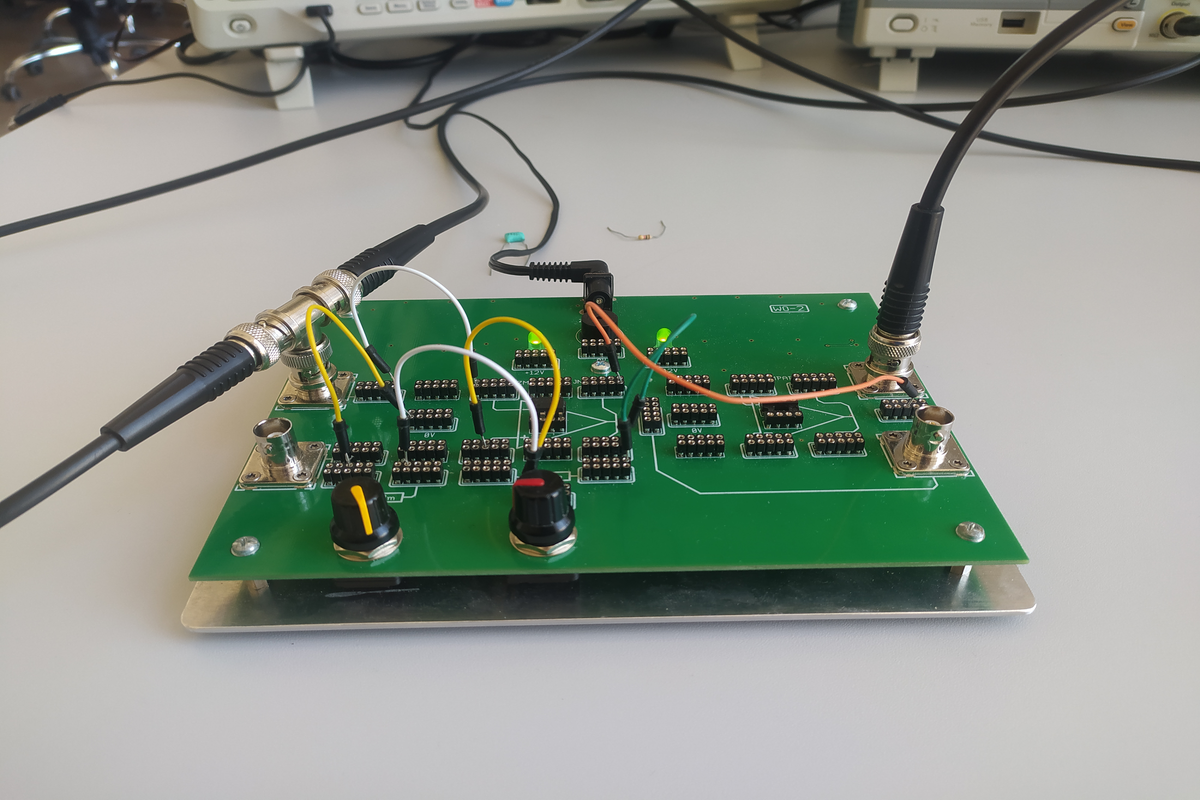
\includegraphics[scale=0.17]{img/phone/1651502036786_scaled.png}
            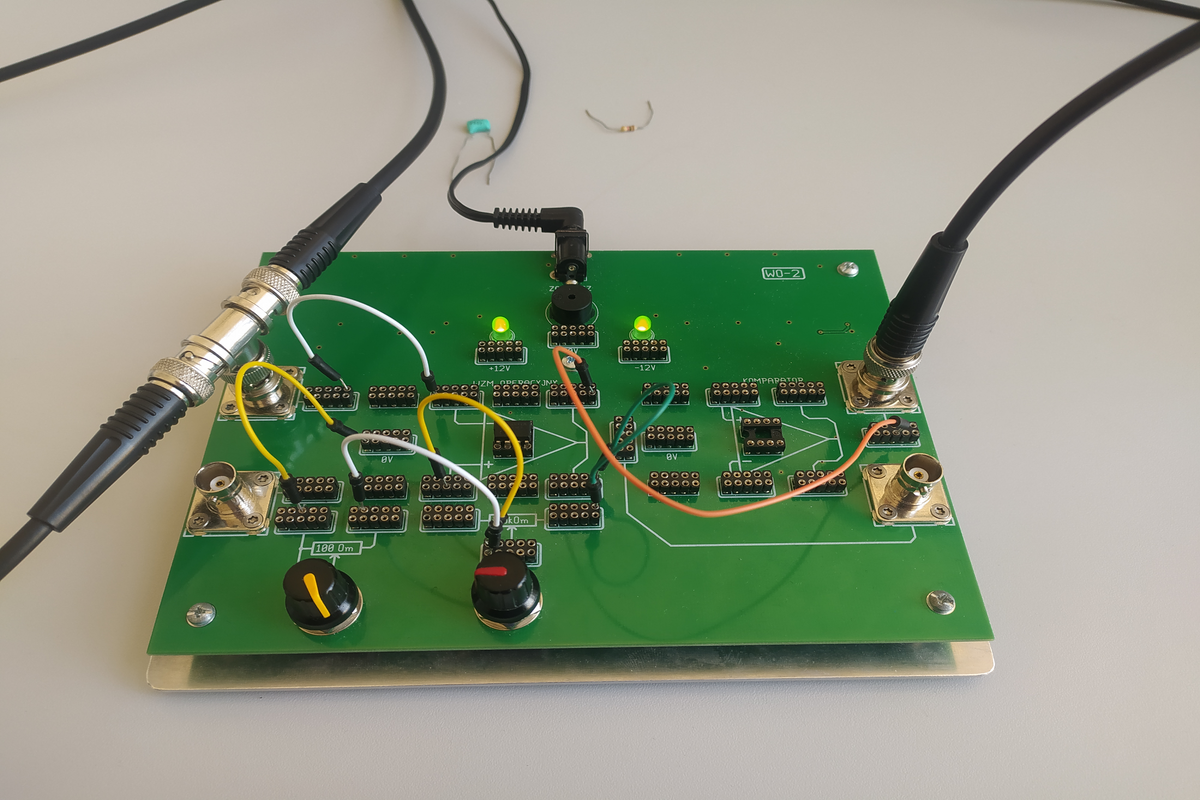
\includegraphics[scale=0.17]{img/phone/1651502036800_scaled.png}
            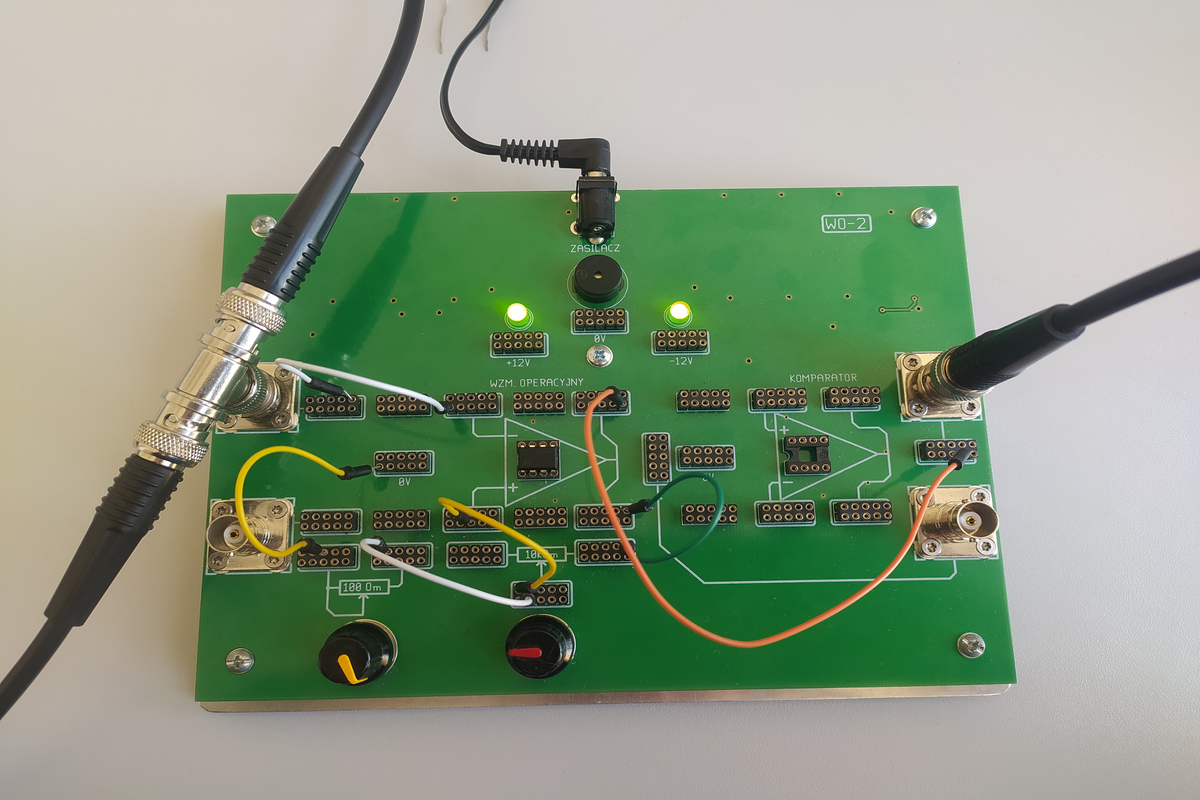
\includegraphics[scale=0.23]{img/phone/1651502036813_scaled.png}
            \caption{Zbudowany przerzutnik Schmidta}
            \label{fig:przerzutnik_schmidta}
        \end{figure}
\end{itemize}

\pagebreak

\section{Przebiegi napięcia wyjściowego}

\begin{itemize}
    \item Przebiegi zostały pobrane przy wartościach oporników równych:
        \begin{gather}
            \label{przerzutnik:R1} R_1 = \textbf{85.9}\boldsymbol{\Omega} \\
            \label{przerzutnik:R2} R_2 = \textbf{1k}\boldsymbol{\Omega}
        \end{gather}
    \item Przebieg napięcia wyjściowego gdy na wejściu podany został sygnał sinusoidalny oraz sygnał trójkątny (oba o wartościach \textbf{1V}, \textbf{1kHz}):
        \begin{figure}[H]
            \centering
            \begin{subfigure}[h]{0.49\textwidth}
                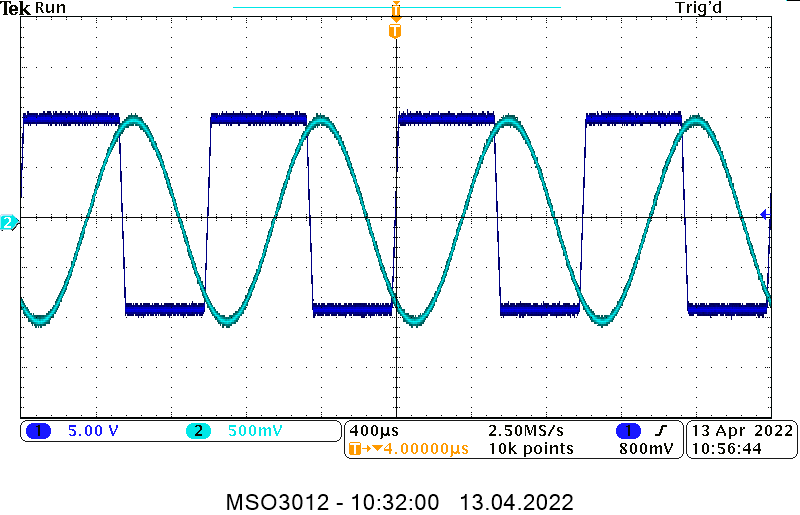
\includegraphics[width=\textwidth]{img/osciloscope/1_4_histereza_przeskok_sin_cropped.png}
                \caption*{Sygnał sinusoidalny}
            \end{subfigure}
            \begin{subfigure}[h]{0.49\textwidth}
                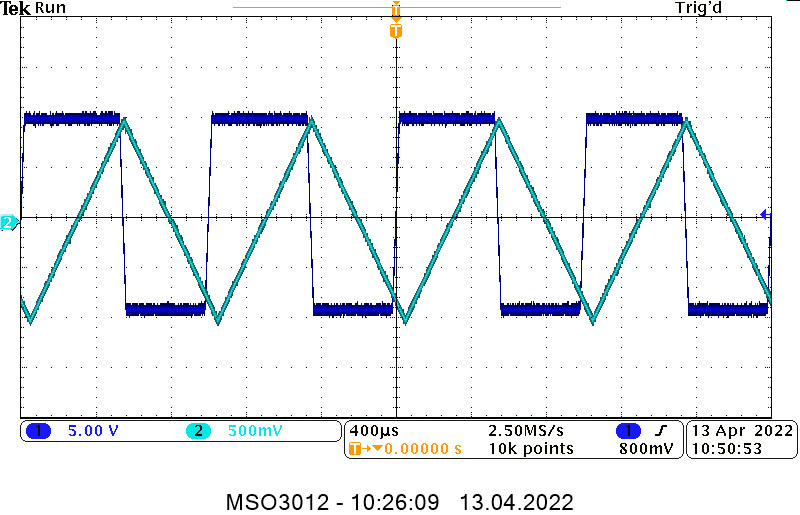
\includegraphics[width=\textwidth]{img/osciloscope/1_4_histereza_przeskok_trojkat_cropped.png}
                \caption*{Sygnał trójkątny}
            \end{subfigure}
        \end{figure}
    \item Teoretyczna reakcja przerzutnika bistabilnego:
        \begin{figure}[H]
            \centering
            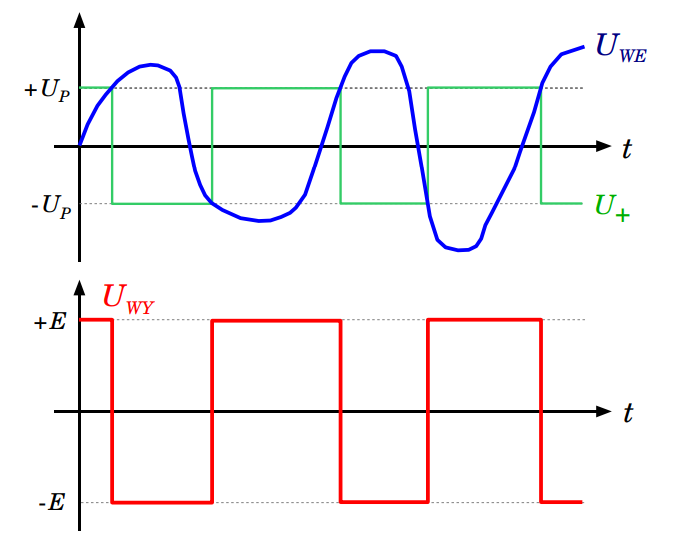
\includegraphics[scale=0.5]{img/theoretical/przerzutnik_reakcja.png}
            \caption{Teoretyczny przebieg}
            \label{fig:my_label}
        \end{figure}
    \item Zbudowany przerzutnik reaguje na zadane sygnały zgodnie z teoretycznymi przewidywaniami.
\end{itemize}

\pagebreak

\section{Histereza}

\begin{itemize}
    \item Do zmierzenia histerezy oraz wykreślenia statycznej charakterystyki układu należało włączyć \textbf{widok XY}.
    \item Teoretyczna pętla histerezy dla układu bistabilnego:
        \begin{figure}[H]
            \centering
            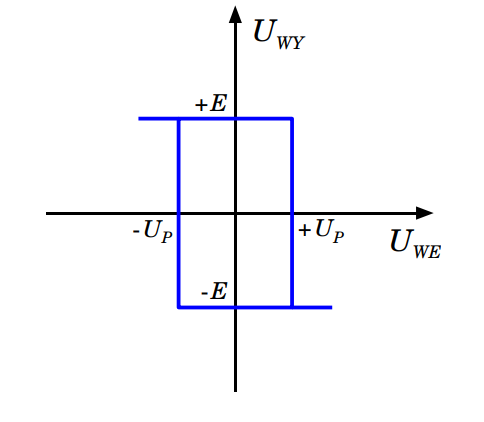
\includegraphics[scale=0.6]{img/theoretical/przerzutnik_histereza.png}
            \caption{Teoretyczna pętla histerezy}
            \label{fig:teoretyczna_histereza}
        \end{figure}
    \item Pętla histerezy wykreślona eksperymentalnie używając oporów (\ref{przerzutnik:R1}, \ref{przerzutnik:R2})
        \begin{figure}[H]
            \centering
            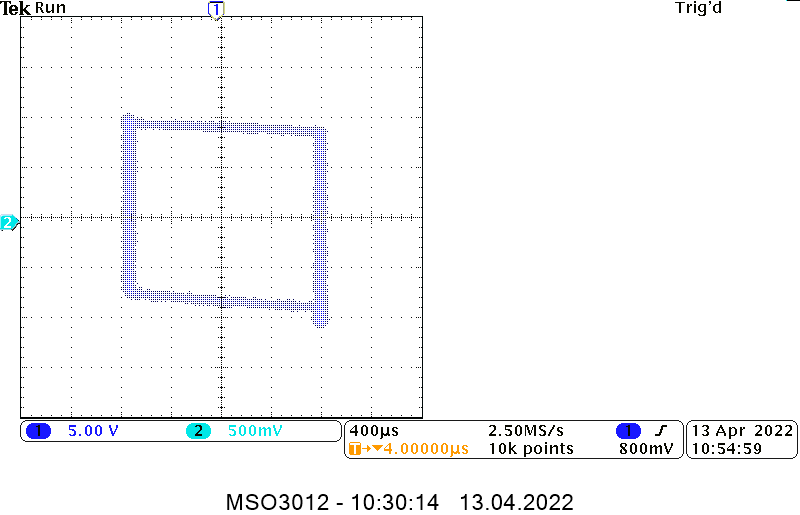
\includegraphics[scale=0.45]{img/osciloscope/1_4_histereza_XY_sin_cropped.png}
            \caption{Sygnał sinusoidalny na wejściu}
            \label{fig:histereza_sin}
        \end{figure}
        \begin{figure}[H]
            \centering
            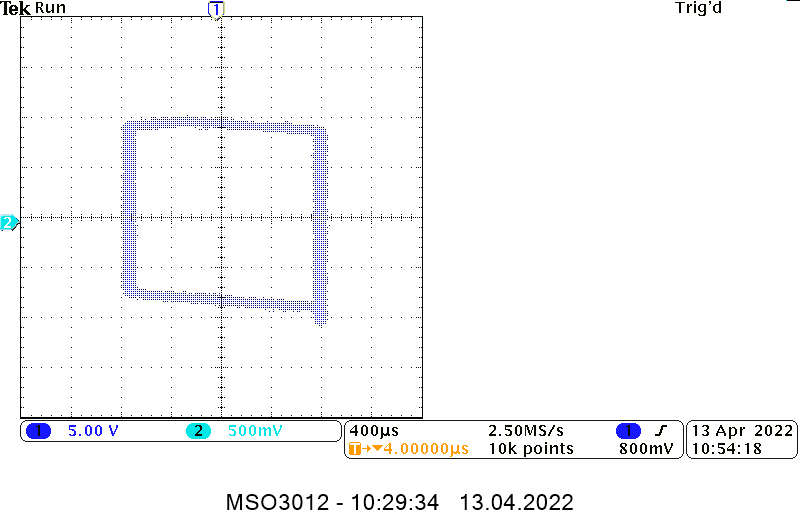
\includegraphics[scale=0.45]{img/osciloscope/1_4_histereza_XY_trojkat_cropped.png}
            \caption{Sygnał trójkątny na wejściu}
            \label{fig:histereza_sin}
        \end{figure}
    \item Teoretyczne wartości dla histerezy:
        \begin{center}
            +E = 11,96V (\ref{pomiar:U+})\\
            -E = -12.02V (\ref{pomiar:U-}) \\
            -$U_p$ = +$U_p$ = 1V 
        \end{center}
        Wartości +/-U = 1, ponieważ przeskok miał następować na 1V
    \item Wartości odczytane z histerezy:
        \begin{center}
            +E = -E $\approx$ 10V (2 odcinki na osi ze skalą równą 5V) \\
            -$U_p$ = +$U_p$ $\approx$ 1V (2 odcinki na osi ze skalą równą 500mV = 0.5V)
        \end{center}
    \item Eksperymentalnie wyznaczona histereza zgadza się z teoretyczną.
    \item Różnica między wartościami teoretycznymi a doświadczalnym mogą wynikać ze źle ustawionej skali bądź osi.
\end{itemize}

\chapter{Propagacja}

\section{Układ}

\begin{itemize}
    \item Schemat układu wraz z rozpiską pinów
        \begin{figure}[H]
            \centering
            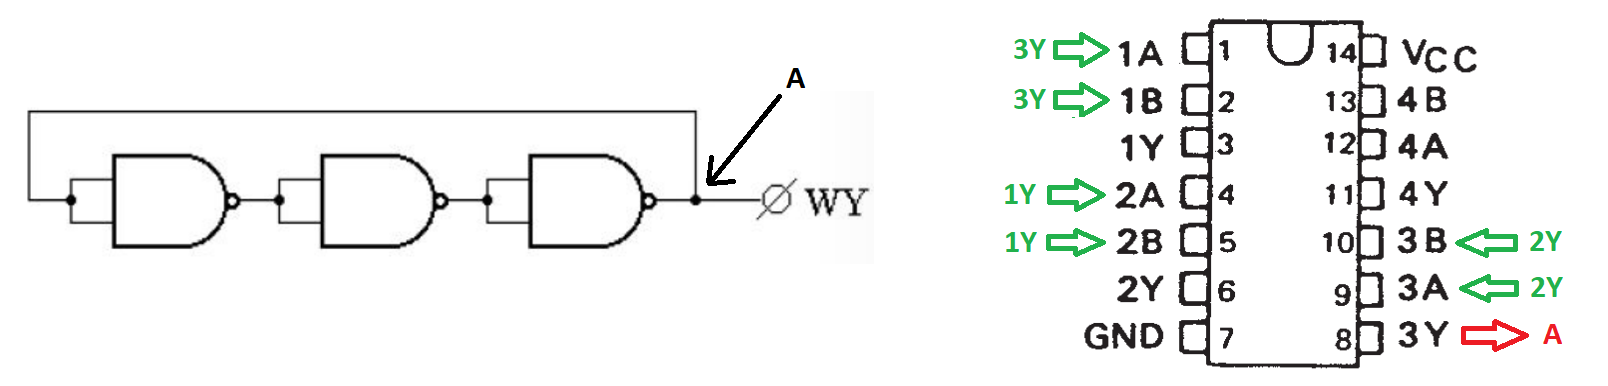
\includegraphics[width=\textwidth]{img/schemes_with_pins/propagacja_w_pins.png}
            \caption{Schemat układu}
            \label{propagacja:schemat}
        \end{figure}
        
    \item Złożony układ:
        \begin{figure}[H]
            \centering
            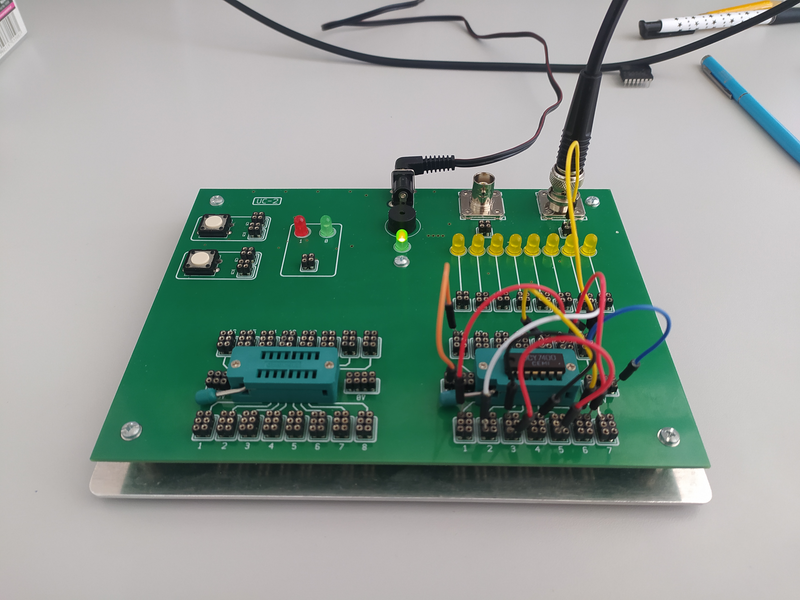
\includegraphics[width=\textwidth]{img/propagacja/1652306732374_scaled.png}
            \caption{Złożony układ}
            \label{propagacja:zlozony_uklad}
        \end{figure}
\end{itemize}

\pagebreak

\section{Pomiary}

\begin{itemize}
    \item Pomiary przeprowadzono dla układu \textbf{TTL 7400}, oraz \textbf{74S00}. Układy posiadają takie samo rozłożenie pinów, dzięki czemu należało wymienić tylko zamocowany układ aby przeprowadzić pomiar dla w/w układów.
    \item Dla układu \textbf{TTL 7400}:
        \begin{figure}[H]
            \centering
            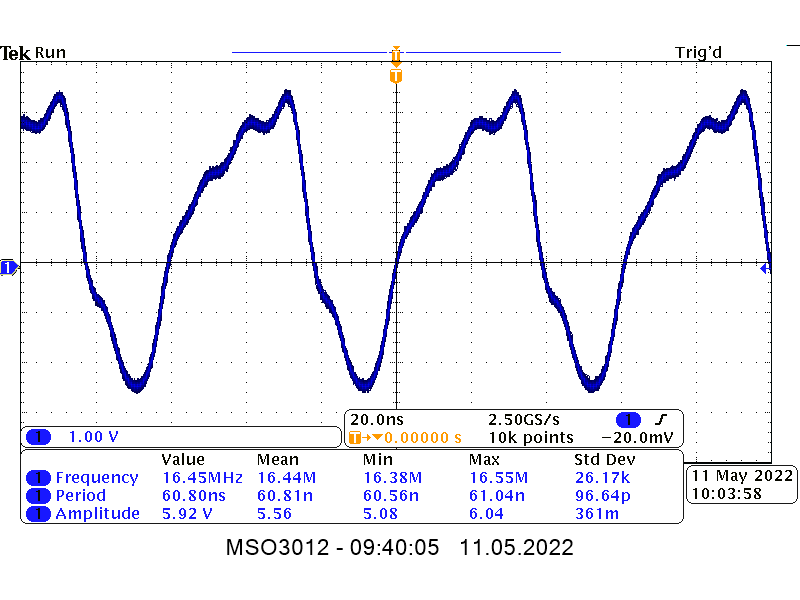
\includegraphics[width=0.7\textwidth]{img/osciloscope/4_propagacja.png}
            \caption{Ściągnięty okres dla układu TTL 7400}
            \label{propagacja:okres_7400}
        \end{figure}
        Teoretyczny średni czas propagacji wynosi (patrz: \ref{propagacja:sredni_czas}, \ref{dokumentacja:7400}):
            \begin{equation}
                t_{teor} = \dfrac{15ns + 22ns}{2} = \textbf{18.5ns}
            \end{equation}
        Okres wyniósł:
            \begin{center}
                $T_{7400}$ = \textbf{60.81ns}
            \end{center}
        Średni czas propagacji:
            \begin{equation}
                t_p = \dfrac{T_{7400}}{6} = \dfrac{60.81ns}{6} \approx \textbf{10.13ns}
            \end{equation}
           
\pagebreak
           
    \item Dla układu \textbf{TTL 74S00}:
        \begin{figure}[H]
            \centering
            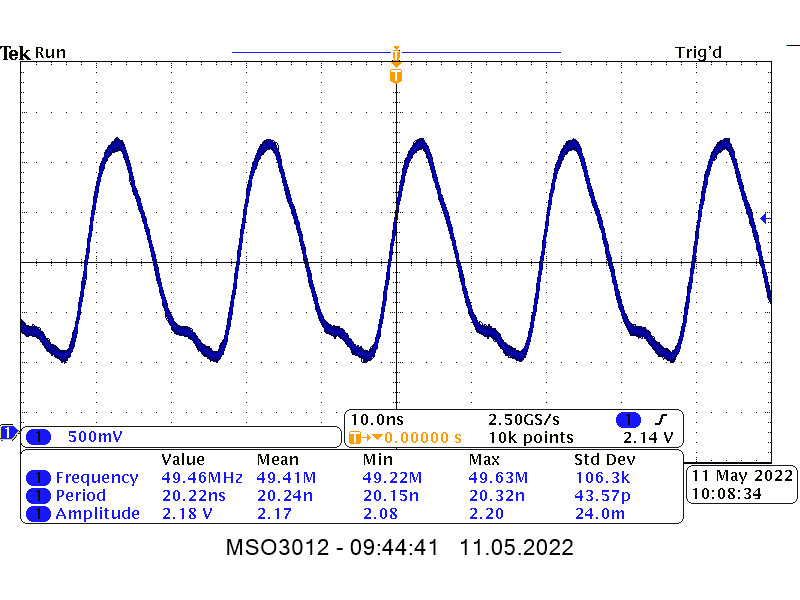
\includegraphics[width=0.7\textwidth]{img/osciloscope/4_propagacja74S00.png}
            \caption{Ściągnięty okres dla układu TTL 74S00}
            \label{propagacja:okres_74S00}
        \end{figure}
        Teoretyczny średni czas propagacji wynosi (patrz: \ref{propagacja:sredni_czas}, \ref{dokumentacja:74S00}):
            \begin{equation}
                t_{teor} = \dfrac{4.5ns + 5ns}{2} = \textbf{4.75ns}
            \end{equation}
        Okres wyniósł:
            \begin{center}
                $T_{74S00}$ = \textbf{20.24ns}
            \end{center}
        Średni czas propagacji:
            \begin{equation}
                t_p = \dfrac{T_{74S00}}{6} = \dfrac{20.24ns}{6} \approx \textbf{3.37ns}
            \end{equation}
\end{itemize}

\chapter{Asynchroniczny przerzutnik R-S}

\begin{itemize}
    \item Schemat razem z rozpiską pinów:
        \begin{figure}[H]
            \centering
            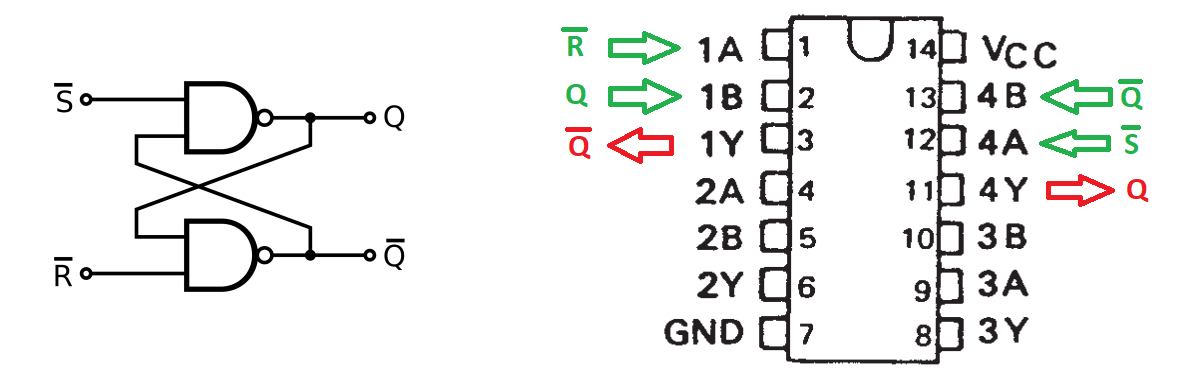
\includegraphics[width=\textwidth]{img/schemes_with_pins/przerzutnik_w_pins.png}
            \label{przerzutnik:schemat_w_pins}
        \end{figure}
    \item Zbudowany przerzutnik:
        \begin{figure}[H]
            \centering
            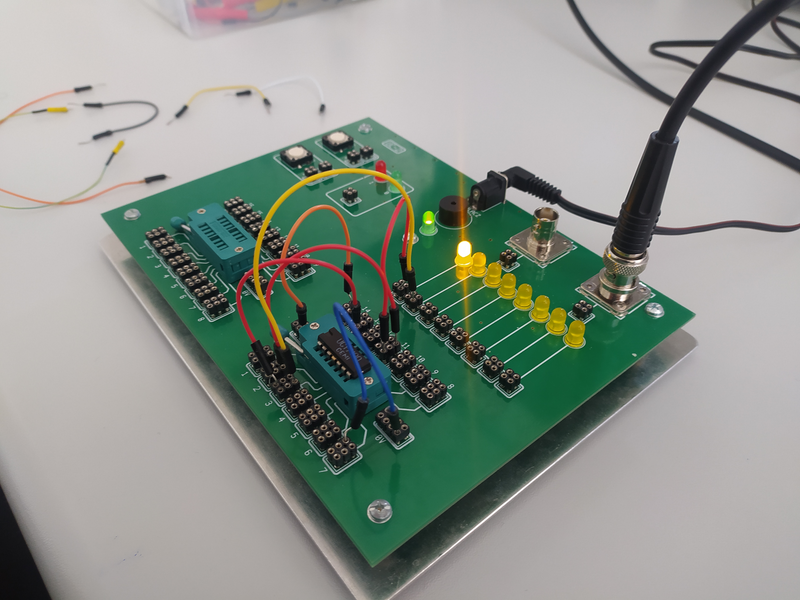
\includegraphics[width=\textwidth]{img/przerzutnik/1652306732322_scaled.png}
            \caption{Zbudowany przerzutnik}
            \label{przerzutnik:zbudowany}
        \end{figure}
        
\pagebreak

    \item Po odłączeniu sygnałów wejściowych przerzutnik pamięta ostatnio zapisany stan:
        \begin{figure}[H]
            \centering
            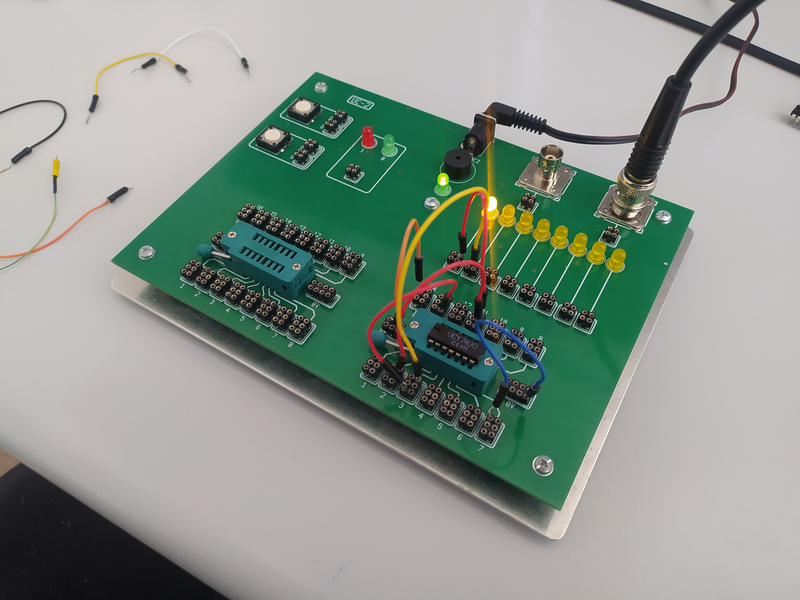
\includegraphics[width=\textwidth]{img/przerzutnik/1652306732331_scaled.png}
            \caption{Zapamiętany stan}
            \label{przerzutnik:pamietanie}
        \end{figure}
        
    \item Przerzutnik zachowuje się zgodnie z przewidywaniami.
\end{itemize}

\chapter{Licznik modulo 10}

\begin{itemize}
    \item Należało zmontować licznik modulo 10 korzystając z układu JK 7493.
    \item Skorzystano z wcześniej zbudowanego licznika modulo 16 (patrz: \autoref{chapter:mod16}).
        \begin{figure}[H]
            \centering
            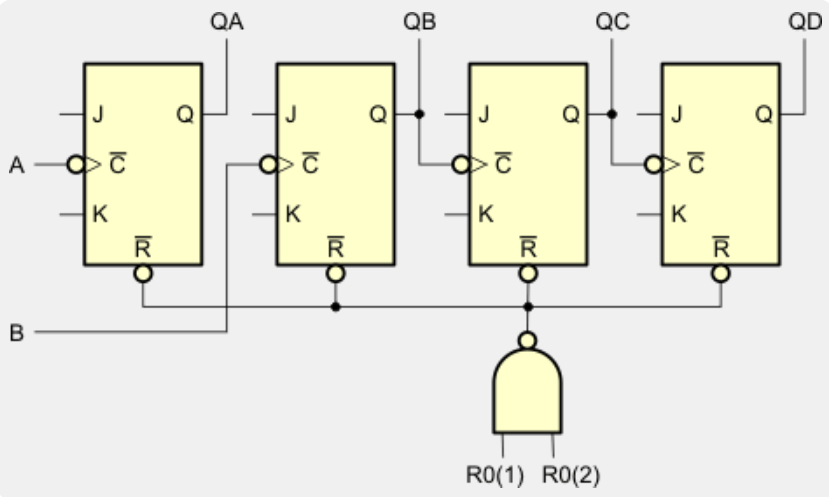
\includegraphics[width=0.7\textwidth]{img/schemes/logic_scheme_7943.png}
            \caption{Schemat logiczny 7493}
            \label{licznik_mod10:schemat_logiczny}
        \end{figure}
    \item Chcąc otrzymać licznik mod 10 należało dodatkowo zadbać o poprawne wywoływanie resetu ($\overline{R}$ na schemacie logicznym (\ref{licznik_mod10:schemat_logiczny})).
    \item Reset powinien następować gdy dostaniemy sekwencję $(1010)_2$ = $(10)_{10}$. Należy wtedy zagwarantować że bramka NAND (patrz: \ref{licznik_mod10:schemat_logiczny}) na swoim wyjściu wygeneruje logiczne \textbf{0} (patrz: \ref{tabela_prawdy:NAND})). Zanegowany sygnał spowoduje reset przerzutników.
    \item Wyjścia licznika QB oraz QD (2 oraz 4 bit) podpięto do bramki NAND (piny 2,3) generującej reset przerzutników.
    \item Wyjścia licznika (QA, QB, QC, QD) zostały wyprowadzone do diod elektroluminescencyjnych     znajdujących się na prawej stronie płytki.
    \item Do wejścia A (pin 14) wpięto sygnał z generatora funkcyjnego o wartościach:
        \begin{center}
            f = 3Hz \\
            $U_{low}$ = 0V \\
            $U_{high}$ = 5V
        \end{center}
    \item LSB (least significant bit) podpięty jest pod pierwszą diodę od lewej (wyjście QA).
        \begin{figure}[H]
            \centering
            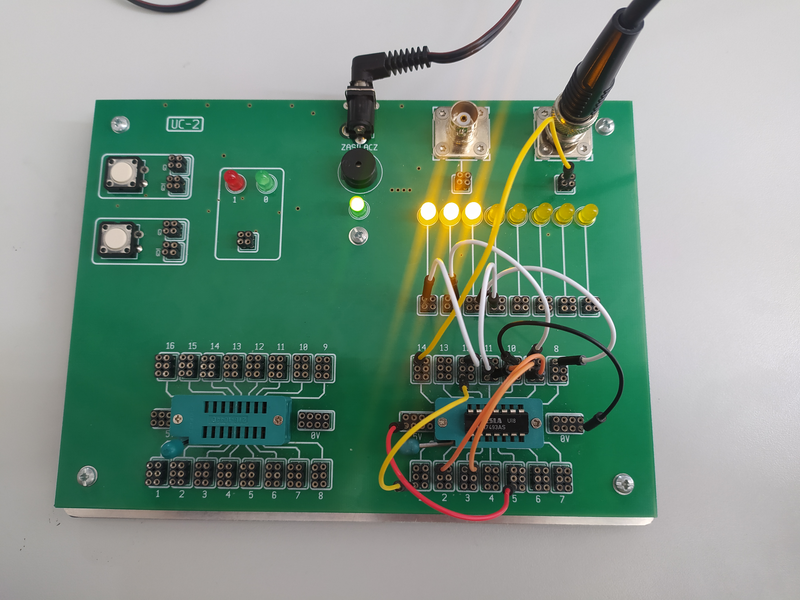
\includegraphics[width=0.7\textwidth]{img/mod10/1653500524710_scaled.png}
            \caption{Zbudowany układ wskazujący $(1110)_2 = (7)_{10}$}
            \label{licznik_mod10:zbudowany_uklad}
        \end{figure}
        
        \begin{figure}[H]
            \centering
            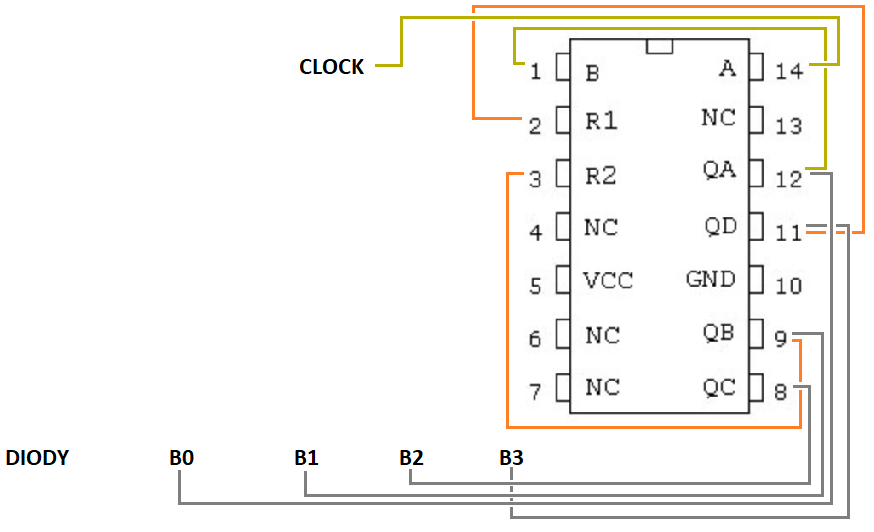
\includegraphics[width=\textwidth]{img/schemes_w_pins/mod10_w_pins.png}
            \caption{Schemat z połączonymi pinami}
            \label{licznik_mod10:schemat_z_pinami}
        \end{figure}
        
    \item Licznik działał \textbf{poprawnie}. Po sekwencji $(1001)_2 = (9)_{10}$ licznik resetował stan do $(0000)_2 = (0)_{10}$. Wciśnięcie impulsatora powodowało reset aktualnego stanu licznika do stanu wyzerowanego $(0000)_2$.
\end{itemize}

\chapter{Rejestry}

\section{Rejestr szeregowy (przesuwający)}

\begin{itemize}
    \item Należało przetestować działanie rejestru szeregowego korzystając z układu 74164. (\ref{link:74164})
        \begin{figure}[H]
            \centering
            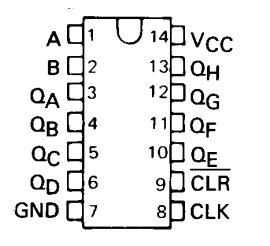
\includegraphics[width=0.5\textwidth]{img/schemes/74164_pins.png}
            \caption{Piny TTL 74164}
            \label{rejestr_szeregowy:piny}
        \end{figure}
    \item Korzystając impulsatorów podajemy wartości na wejście A oraz B rejestru szeregowego.
    \item Wejście zegara (pin 8) obsługujemy za pomocą generatora funkcyjnego generującego sygnał o zadanych wartościach:
        \begin{center}
            f = 1Hz \\
            $U_{low}$ = 0V \\
            $U_{high}$ = 5V
        \end{center}
    \item Wyjścia rejestru QA-QH (piny 3,4,5,6,10,11,12,13) zostały wyprowadzone do diod elektroluminescencyjnych znajdujących się na prawej stronie płytki.
        \begin{figure}[H]
            \centering
            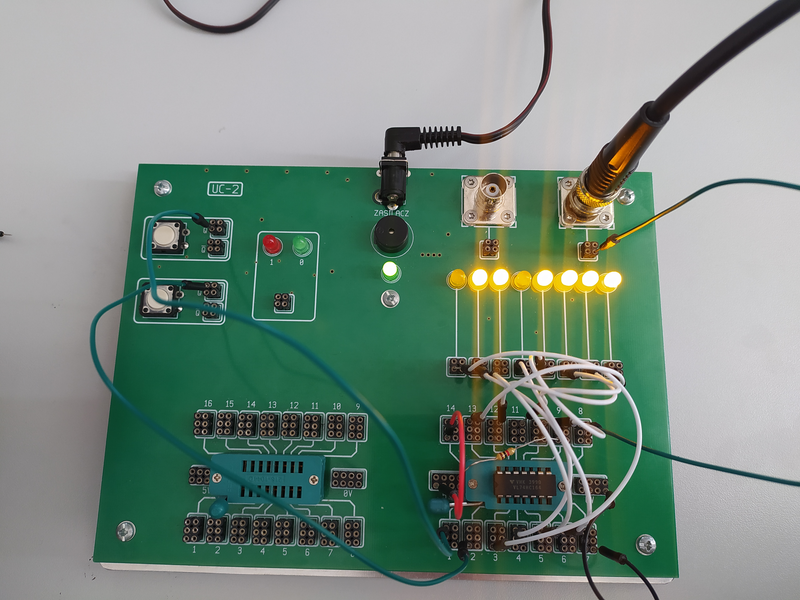
\includegraphics[width=0.7\textwidth]{img/74164/1653500524524_scaled.png}
            \caption{Zbudowany rejestr szeregowy}
            \label{rejestr_szeregowy:zbudowany}
        \end{figure}
        
        \begin{figure}[H]
            \centering
            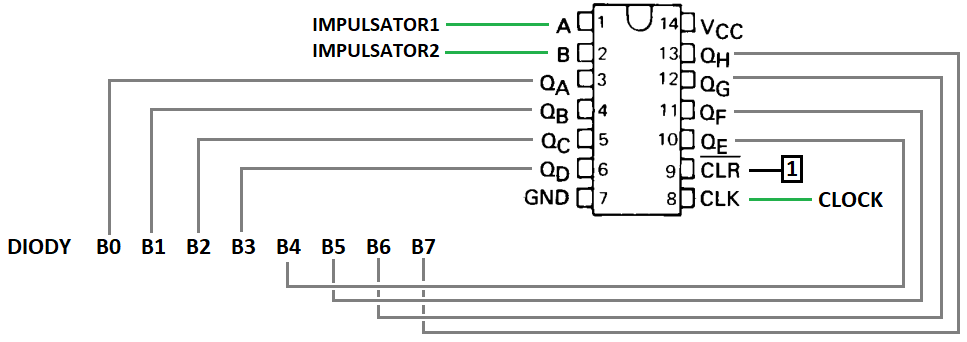
\includegraphics[width=\textwidth]{img/schemes_w_pins/74164_w_pins.png}
            \caption{Schemat z połączonymi pinami}
            \label{rejestr_szeregowy:schemat_z_pinami}
        \end{figure}
        
    \item Podczas jednoczesnego wysłania impulsu z impulsatora 1 oraz 2 (wejścia A, B) na rejestrze pojawia się logiczna 1, która przesuwa się do kolejnej pozycji razem z każdym tyknięciem zegara.
    \item Zbudowany rejestr szeregowy działał \textbf{poprawnie}.
\end{itemize}

\pagebreak

\section{Rejestr równoległy (buforowy)}

\begin{itemize}
    \item Należało przetestować działanie rejestru równoległego korzystając z układu 74165. (\ref{link:74165})
        \begin{figure}[H]
            \centering
            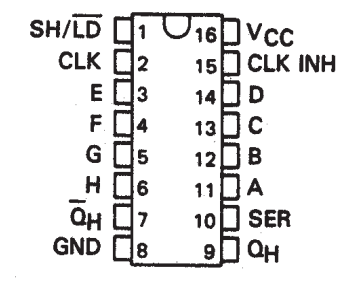
\includegraphics[width=0.5\textwidth]{img/schemes/74165_pins.png}
            \caption{Piny TTL 74165}
            \label{rejestr_rownolegly:piny}
        \end{figure}
    \item Korzystając impulsatorów podano wartości na 2 z 8 pinów wejściowych (B oraz C).
    \item Wejście zegara (pin 8) obsługujemy za pomocą generatora funkcyjnego generującego sygnał o zadanych wartościach:
        \begin{center}
            f = 1Hz \\
            $U_{low}$ = 0V \\
            $U_{high}$ = 5V
        \end{center}
    \item Wyjście rejestru QH zostało wyprowadzone do testera logicznego.
    \item Wejście SH/LD – wejście sterujące ładowaniem danych lub przesuwaniem informacji w rejestrze. \\
        W stanie niskim do przerzutników rejestru zostaje zapisana informacja z wejść danych A...H. \\ 
        W stanie wysokim informacja w rejestrze może być przesuwana. \\
        \textbf{Do wejścia zostało podpięte logiczne 0 (stan niski).}
    \item Wejście CLK INH – w stanie wysokim blokuje sygnał zegarowy, informacja nie jest przesuwana w rejestrze. \\
        \textbf{Do wejścia zostało podpięte logiczne 0 (stan niski).}
        \begin{figure}[H]
            \centering
            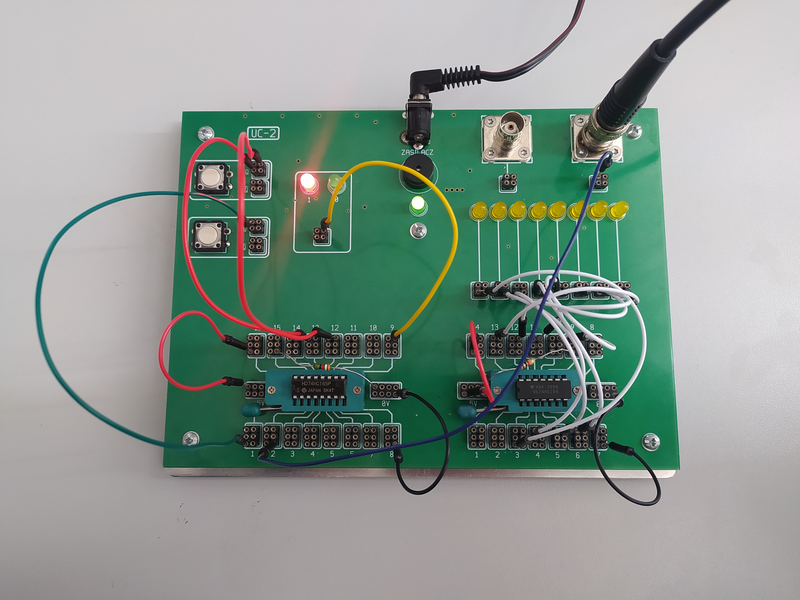
\includegraphics[width=0.7\textwidth]{img/74165/1653500524502_scaled.png}
            \caption{Zbudowany rejestr równoległy}
            \label{rejestr_rownolegly:zbudowany}
        \end{figure}
        
        \begin{figure}[H]
            \centering
            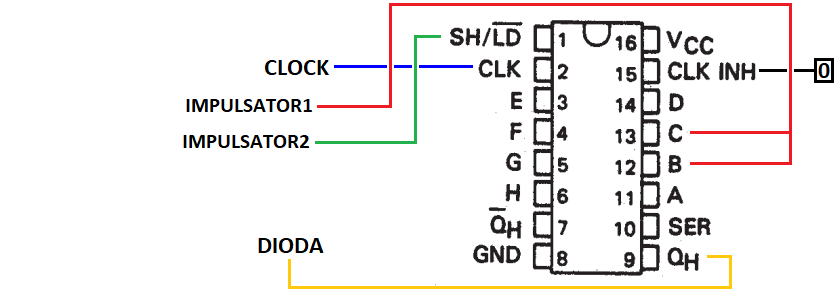
\includegraphics[width=\textwidth]{img/schemes_w_pins/74165_w_pins.png}
            \caption{Schemat z połączonymi pinami}
            \label{rejestr_rownolegly:schemat_z_pinami}
        \end{figure}
        
    \item Z każdym taktem zegara wyświetlany był aktualny bit na rejestrze, po czym wyświetlany był następny bit w rejestrze.
    \item Zbudowany rejestr szeregowy działał \textbf{poprawnie}.
\end{itemize}

\chapter{Podsumowanie}

\section{Opis doświadczeń}
\begin{itemize}
    \item Celem przeprowadzonych doświadczeń było zbadanie charakterystyk amplitudowych oraz fazowych układów CR, RC oraz CLR.
    \item Dodatkowo badano reakcje układów CR oraz RC na podanie fal prostokątnych oraz trójkątnych.
    \item Obliczono teoretyczne wartości częstotliwości granicznych oraz zestawiono je z eksperymentalnie wyznaczonymi danymi.
    \item Eksperymentalne dane przedstawiono w postaci tabeli oraz na wykresie wraz z teoretycznymi funkcjami.
    \item Różnice między wartościami empirycznymi a teoretycznymi były niewielkie, najpewniej spowodowane były krótkim okresem stabilizacji pomiarów oscyloskopu między poszczególnymi pomiarami oraz przybliżeniem obliczeń teoretycznych.
\end{itemize}

\section{Literatura}

\begin{enumerate}
    \item Studencka Pracownia Elektroniczna \\
    Wykład "Wstęp do elektroniki" dr. hab. Janusza Brzychczyka \\
    \url{http://zefir.if.uj.edu.pl/pracownia_el/jb_w4.pdf}
\end{enumerate}

\end{document}